\newpage
\section{Системные вызовы процессов реального времени}

Для изучения системных вызовов sched\_setparam, sched\_getparam и sched\_rr\_get\_interval целесообразно рассмотреть всю группу системных вызовов, позволяющих процессу менять его дисциплину планирования и, в частности, становиться процессом реального времени. Процесс должен иметь способность CAP\_SYS\_NICE (т.е. способностью изменять приоритет чужих процессов), чтобы модифицировать значения полей rt\_priority и policy у дескриптора любого процесса, включая собственный.

Системный вызов \textbf{sched\_getscheduler} запрашивает политику планирования, действующую в отношении процесса, идентифицируемого параметром pid. Если значение pid во время вызова равен 0, считывается политика вызвавшего процесса. В случае успеха системный вызов возвращает политику sched\_fifo, sched\_rr или sched\_normal (последняя также называется sched\_other). Соответствующая служебная процедура sys\_sched\_getscheduier вызывает функцию find\_process\_by\_pid, которая находит дескриптор процесса по переданному значению pid и возвращает значение его поля policy.

Системный вызов \textbf{sched\_setscheduier} устанавливает как политику планирования, так и соответствующие параметры для процесса, идентифицируемого параметром pid. Как и в случае с sched\_getscheduler, если pid равен 0, то устанавливаются параметры планировщика, применяемые к вызвавшему процессу. Соответствующая служебная процедура sys\_sched\_setscheduler вызывает функцию do\_sched\_setscheduler. Эта функция проверяет допустимость политики планирования, определяемой параметром policy, и нового приоритета, определяемого параметром param->sched\_priority. Она также проверяет, есть ли у процесса способность CAP\_SYS\_NICE, или наличие прав суперпользователя у его владельца. Если все в порядке, она удаляет процесс из очереди на выполнение (если он выполняемый), обновляет статический и динамический приоритеты и приоритет реального времени у процесса, возвращает процесс в очередь на выполнение и, если необходимо, вызывает функцию resched\_task для вытеснения текущего процесса, принадлежащего данной очереди.

Системный вызов \textbf{sched\_getparam} читает параметры процесса, идентифицируемого параметром pid. Если pid равен 0, считываются параметры текущего процесса. Соответствующая служебная процедура sys\_sched\_getparam, как и следует ожидать, находит указатель на дескриптор процесса по параметру
pid, сохраняет поле rt\_priority в локальной переменной типа sched\_param и вызывает функцию copy\_to\_user, чтобы скопировать это значение в адресное пространство процесса, по адресу, заданному параметром param.

Системный вызов \textbf{sched\_setparam} аналогичен вызову sched\_setscheduler, различие состоит в том, что sched\_setparam не позволяет вызвавшему процессу задавать значение поля policy. Соответствующая служебная процедура sys\_sched\_setparam вызывает функцию do\_sched\_setscheduler практически с теми же параметрами, что и служебная процедура sys\_sched\_setscheduler.

Системный вызов \textbf{sched\_yieido} позволяет процессу добровольно освободить процессор без приостановки своего выполнения. Процесс остается в состоянии TASK\_RUNNING, а планировщик заносит его либо в набор процессов с истекшими квантами времени (если это обычный процесс), либо в конец списка в очереди на выполнение (если это процесс реального времени). Затем вызывается функция schedule. В результате у других процессов с тем же динамическим приоритетом появляется возможность поработать. Данный вызов используется, в основном, процессами реального времени, принадлежащими классу SCHED\_FIFO.

Системные вызовы \textbf{sched\_get\_priority\_min} и \textbf{sched\_get\_priority\_max} возвращают, соответственно, минимальный и максимальный статический приоритет реального времени, который может быть использован при проведении политики планирования, идентифицируемой параметром policy. Служебная процедура sys\_sched\_get\_priority\_min возвращает 1, если текущий процесс является процессом реального времени, и 0 в противном случае. Служебная процедура sys\_sched\_get\_priority\_max возвращает 99 (наивысший приоритет), если текущий процесс является процессом реального времени, и 0 в противном случае.

Системный вызов \textbf{sched\_rr\_get\_interval} записывает в структуру, хранящуюся в адресном пространстве режима пользователя, квант времени, соответствующий круговому принципу работы, для процесса реального времени, идентифицируемого параметром pid. Если pid равен 0, системный вызов записывает квант времени текущего процесса. Как и в предыдущих примерах, соответствующая служебная процедура sys\_sched\_rr\_get\_interval вызывает функцию find\_process\_by\_pid, для получения дескриптора процесса по значению pid. Затем она преобразует базовый квант времени выбранного процесса в секунды и наносекунды, и копирует эти числа в структуру пользовательского режима. В соответствии с соглашением, временной квант процесса реального времени, принадлежащего классу "первым вошел — первым вышел", равен нулю.

Рассмотренные системные вызовы позволяют реализовать различные расширения реального времени POSIX.1b начиная с ядра Linux версии 2.6\cite{Raghavan}. Для определения задачи реального времени в Linux есть три основных параметра:
\begin{itemize}
\item Класс планирования
\item Приоритет процесса
\item Интервал времени
\end{itemize}
 
\textbf{Планировщик} Linux предлагает три класса планирования, два для приложений реального времени и один для приложений не реального времени. Этими тремя классами являются:
\begin{itemize}
\item SCHED\_FIFO: политика планирования реального времени первый вошёл, первый вышел (First-In First-Out). Алгоритм планирования не использует никаких интервалов времени. Процесс SCHED\_FIFO выполняется до завершения, если он не заблокирован запросом ввода/вывода, вытеснен высокоприоритетным процессом, или он добровольно отказывается от процессора. Следует обратить внимание на следующие моменты:
\begin{itemize}
\item Процесс SCHED\_FIFO, который был вытеснен другим процессом более высокого приоритета, остаётся во главе списка с его приоритетом и возобновит выполнение, как только все процессы с более высоким приоритетом будут вновь заблокированы.
\item Когда процесс SCHED\_FIFO готов к работе (например, после пробуждения от операции блокировки), он будет вставлен в конец списка с его приоритетом.
\item Вызов sched\_setscheduler или sched\_setparam поставит процесс SCHED\_FIFO в начало списка. Как следствие, это может вытеснить работающий в данный момент процесс, если его приоритет такой же, как и у работающего процесса.
\end{itemize}
\item SCHED\_RR: циклическая (Round-Robin) политика планирования реального времени. Она похожа на SCHED\_FIFO с той лишь разницей, что процессу SCHED\_RR разрешено работать как максимум время кванта. Если процесс SCHED\_RR исчерпывает свой квант времени, он помещается в конец списка с его приоритетом. Процесс SCHED\_RR, который был вытеснен процессом с более высоким приоритетом, завершит оставшуюся часть своего кванта времени после возобновления выполнения.
\item SCHED\_OTHER: стандартный планировщик Linux с разделением времени для процессов, работающих не в реальном времени.
\end{itemize}

Диапазоны \textbf{приоритетов} для различных политик планирования показаны в Таблице 1.

\begin{table}
\caption{Диапазоны приоритетов различных политик планирования}
\centering
\begin{tabular}{|c|c|}
\hline 
Класс планирования & Диапазон приоритетов \\ 
\hline 
SCHED\_OTHER & 0 \\ 
\hline 
SCHED\_FIFO & 1 - 99 \\ 
\hline 
SCHED\_RR & 1 - 99 \\ 
\hline 
\end{tabular}
\end{table}

Ядро позволяет значению nice быть установленным как для процесса SCHED\_RR или SCHED\_FIFO, но это не будет иметь никакого влияния на планирование, пока задача выполняется с классом SCHED\_OTHER.

Точка зрения ядра на приоритеты процессов отличается от точки зрения процессов. Соответствие между приоритетами пользовательского пространства и пространства ядра для задач реального времени в ядре показывает Рисунок 1.

\begin{figure}[h!]
\centering
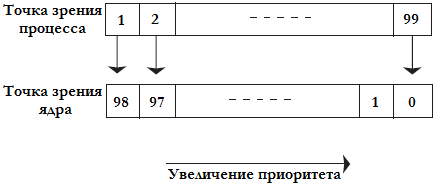
\includegraphics[scale=1]{res/pic001}
\caption{Отображение приоритетов пользовательского уровня на пространство ядра}
\end{figure}

Для ядра низкое значение означает высокий приоритет. Приоритеты реального времени в ядро находятся в диапазоне от 0 до 98. Таким образом, пользовательский приоритет 1 связывается с приоритетом ядра 98, приоритет 2 с 97, и так далее.

\textbf{Интервал времени} действителен только для процессов SCHED\_RR. Процессы SCHED\_FIFO можно рассматривать как имеющие бесконечный интервал времени. Так что это обсуждение касается только процессов SCHED\_RR.

Linux устанавливает минимальный интервал времени для процесса как 10 мс, интервал времени по умолчанию как 100 мс, а максимальный интервал времени как 200 мс. Интервалы времени заполняются вновь после их окончания\cite{Raghavan}. В версии 2.6 интервал времени процесса рассчитывается так:

\begin{Verbatim}[frame=single]
#define MIN_TIMESLICE (10)
#define MAX_TIMESLICE (200)
#define MAX_PRIO (139)   // MAX внутренний приоритет ядра
#define MAX_USER_PRIO 39 // MAX nice при переводе к положительной шкале

/* ‘p’ это структура задач процесса */
#define BASE_TIMESLICE(p) \
   (MIN_TIMESLICE + ((MAX_TIMESLICE - MIN_TIMESLICE) *
   (MAX_PRIO-1 - (p)->static_prio) / (MAX_USER_PRIO-1)))
\end{Verbatim}

Можно заметить, что static\_prio содержит значение nice для процесса. Ядро преобразует диапазон nice c -20 до +19 во внутренний диапазон nice  в ядре от 100 до 139. Поле nice процесса конвертируется в такой масштаб и сохраняется в static\_prio. Таким образом, значение nice -20 соответствует static\_prio 100, а +19 для nice, static\_prio 139. Наконец, интервал времени процесса возвращает функция task\_timeslice.

\begin{Verbatim}[frame=single]
static inline unsigned int task_timeslice(task_t *p) {
  return BASE_TIMESLICE(p);
}
\end{Verbatim}

Отметим, что static\_prio является единственной переменной в расчёте интервала времени. Таким образом, можно сделать некоторые важные выводы:
\begin{itemize}
\item Все процессы SCHED\_RR выполняются по умолчанию с интервалом времени в 100 мс, поскольку они обычно имеют значение nice, равное 0.
\item При значении nice -20 процесс SCHED\_RR получит интервал времени 200 мс, а при nice +19 процесс SCHED\_RR получит  интервал времени 10 мс. Таким образом, значение nice может быть использовано для управления выделением интервала времени для процессов SCHED\_RR.
\item Чем меньше значение nice (то есть, приоритет более высокий), тем больше интервал времени.
\end{itemize}
 